\par 
La \textbf{géotechnique} est l’ensemble des 
activités liées aux applications de la mécanique des sols, de la mécanique 
des roches et de la géologie de l’ingénieur\footnote{
    Définition selon l’Union syndicale géotechnique accessible via ce lien: 
    \url{http://u-s-g.org/profession-geotechnicien.asp?idpage=1}}.
Au cours d'un projet d'aménagement, dans le but d'assurer  la fiabilité et la durabilité
des ouvrages, le constructeur est dans l'obligation de prendre en compte
la nature du sous-sol du site où il est prévu de construire.

Il s'agit en fait d'adapter le projet au site envisagé.
\par
La mission du géotechnicien consiste principalement à:
\begin{itemize}
    \item définir les cadres géologique, hydrogéologique et topographique 
    du site étudié ;
    \item définir les aléas existants vis-à-vis des risques naturels : 
    détection des cavités, stabilité général d’un site (par rapport au 
    glissement de terrain par exemple), sismicité.
    \item définir les terrassements : faisabilité, réemploi des matériaux, 
    tenus des talus et parois des fouilles ;
    \item définir l’influence des circulations d’eaux souterraines, 
    agressivité de l’eau vis-à-vis des bétons ;
    \item définir comment la nature et la répartition des 
    formations géologiques pourrait influencer la réalisation des travaux et la conception 
    de l’ouvrage.
\end{itemize}
\paragraph{}
En général, le géotechnicien résume sa mission dans un rapport.
Ce rapport comprend les résulatats des différents tests (Figure \ref{fig:test_penetrometrique}) réalisés : essais de pénétration, forages, essais de laboratoire,
essais géophysiques, etc.
Ce rapport est rédigé non seulement dans le but d’informer le client sur la nature des interventions
, mais aussi d’exposer les principaux résultats des tests recueillis, de façon à mener à bien
l’exécution des projets.
\par
La zone d'étude de ce projet correspond à Haïti (Figure \ref{fig:haiti}) .
Cette île située dans les Caraïbes a une superficie de  \SI{27750}{\kilo\metre\squared}.
L'importance des données géotechiques s'est montrée incontournable dans ce pays surtout 
après un séisme en Janvier 2010.

\paragraph{Un événement mémorable, une leçon à tirer!!}
Vulgairement appelé Goudougoudou, un séisme de magnitude 7, sur l'échelle de Richter, 
a fait de grands ravages sur l'île. Les pertes enregistrées, tant en vie humaines qu'en biens
matérielles, ne faisaient que refléter l'ignorance de certains, et le laisser-aller des autres. 
Des bâtiments construits défavorablement, des ravines devenues des villages ou simplement des 
constructions effectuées sur un sol non adéquats, telles étaient les causes majeures de ces 
pertes. Par exemple, une maison a simplement été victime d'un glissement de terrain \textbf{Il 
serait interessant de trouver l image adequate}. Avec une 
étude de sol et des données géotechniques adéquates, un ingénieur pourrait orienter son travail
en connaissance de cause. Par conséquent, depuis maintenant une bonne décennie, les demandes
se multiplient pour l'accès à ces informations.  

\begin{figure}
    \centering
    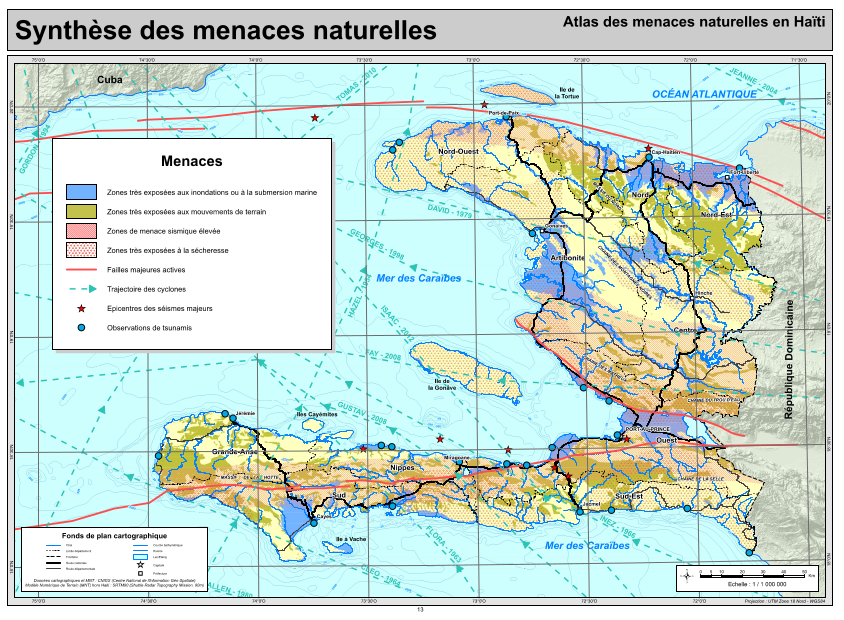
\includegraphics[width=1\textwidth]{images/Contexte/haiti.png}
    \caption{Cartographie d'Haïti, Synthèse des menaces naturelles.}
    \label{fig:haiti}
\end{figure}

\begin{figure}
    \centering
    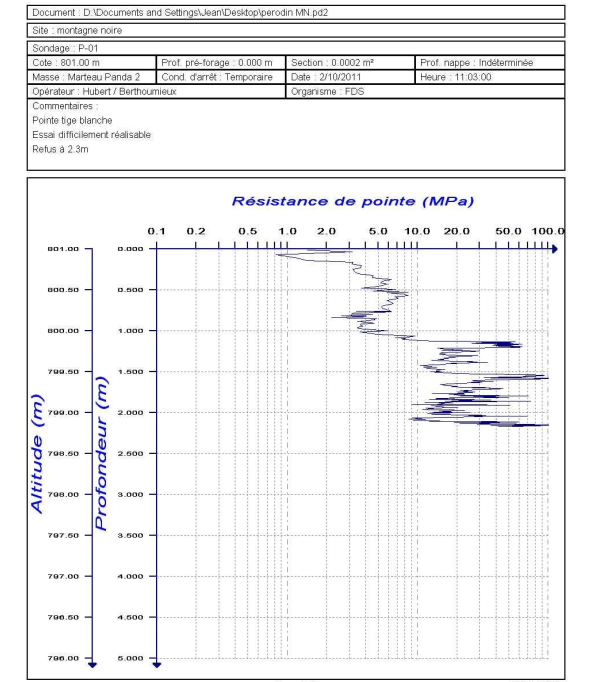
\includegraphics[width=1\textwidth]{images/Contexte/penetrographe.png}
    \caption{Exemple de résultat d'un essai pénétrométrique}
    \label{fig:test_penetrometrique}
\end{figure}
